\documentclass[11pt]{article}
\usepackage{latexsym}
\usepackage{amsmath}
\usepackage{amssymb}
\usepackage{amsthm}
\usepackage{epsfig}
\usepackage[tight]{subfigure}

\usepackage{amsmath}

\DeclareMathOperator*{\minimize}{min}
\DeclareMathOperator*{\maximize}{max}

\usepackage{algorithm}
 %on linux you may need to run sudo apt-get install texlive-full to install algorithm.sys
\usepackage{algorithmic}

\usepackage{verbatim}

\newcommand{\handout}[5]{
  \noindent
  \begin{center}
  \framebox{
    \vbox{
      \hbox to 5.78in { {#1} \hfill #2 }
      \vspace{4mm}
      \hbox to 5.78in { {\Large \hfill #5  \hfill} }
      \vspace{2mm}
      \hbox to 5.78in { {\em #3 \hfill #4} }
    }
  }
  \end{center}
  \vspace*{4mm}
}

\newcommand{\lecture}[5]{\handout{#1}{#2}{#3}{#4}{#5}}
\newcommand{\collision}[0]{\mathrm{collision}}
\newcommand{\nocollision}[0]{\overline{\collision}}

\newcommand*{\QED}{\hfill\ensuremath{\square}}

\newtheorem{theorem}{Theorem}
\newtheorem{corollary}[theorem]{Corollary}
\newtheorem{lemma}[theorem]{Lemma}
\newtheorem{observation}[theorem]{Observation}
\newtheorem{proposition}[theorem]{Proposition}
\newtheorem{definition}[theorem]{Definition}
\newtheorem{claim}[theorem]{Claim}
\newtheorem{fact}[theorem]{Fact}
\newtheorem{assumption}[theorem]{Assumption}
\newtheorem{note}[theorem]{Note}

% 1-inch margins, from fullpage.sty by H.Partl, Version 2, Dec. 15, 1988.
\topmargin 0pt
\advance \topmargin by -\headheight
\advance \topmargin by -\headsep
\textheight 8.9in
\oddsidemargin 0pt
\evensidemargin \oddsidemargin
\marginparwidth 0.5in
\textwidth 6.5in

\parindent 0in
\parskip 1.5ex
%\renewcommand{\baselinestretch}{1.25}

\begin{document}

\lecture{Statistical Techniques in Robotics (16-831, S22)}{Lecture \#02
  (Monday, January 24)}{Lecturer: Kris Kitani}{Scribes: Feng Xiang, Husam Wadi}{PWEA \& Greedy/Consistent Algorithm}

\section{Review}
In the last lecture, we went over course logistics and discussed how to analyze and break down a robot learning problem to determine the best approach. Statistical robotics, from a high-level standpoint, pertains to the methods used to use and process high amounts of data to solve robotics problems. These statistical problems were broken down into the categories shown in \ref{img:categories} shown below:

\begin{figure}[H]
\centering
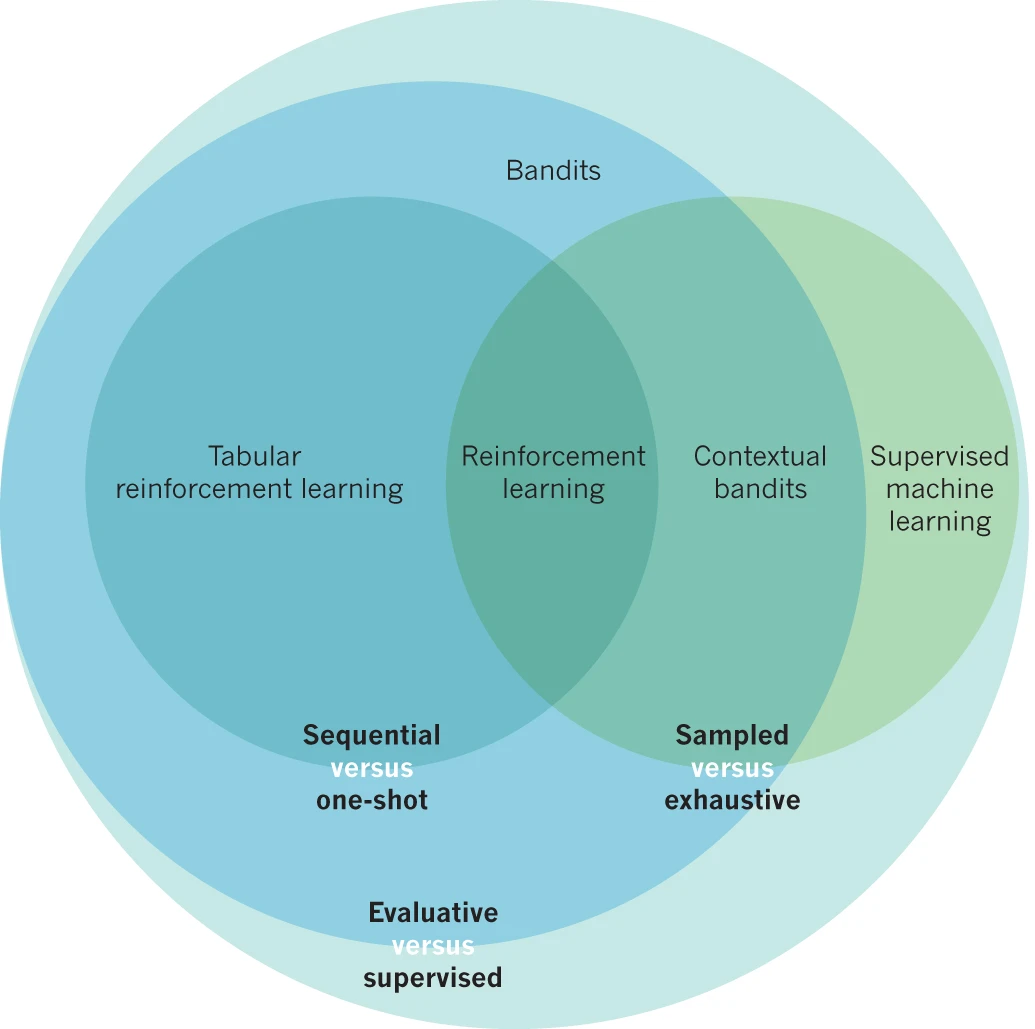
\includegraphics[width=4.5in]{categories.png}
\caption{Categories of robot learning problems\cite{Akshay2021}.}
\label{img:categories}
\end{figure}

%This section serves as a review of the previous lecture and any other context required to frame the content of the current lecture. 

%You may format the scribes in any way you like, aside from changing font style, size and page format. Please use subsections and paragraphs to increase the readability of your notes.

%Length requirement 1-2 pages.
        
\subsection{Classifying Learning Problems}
In the field of statistical robots, there are a plethora of learning approaches to use. A learning problem can be framed into three major learning approach areas\cite{littman2015reinforcement}:

\begin{enumerate}
    \item exhaustive vs sampled feedback
    \begin{itemize}
        \item exhaustive: All data being seen will cover the learner's observation/state/action space.
        \item sampled: Learner is exposed to only a sub-set of the observation/state/action space.
    \end{itemize}
    \item instructive vs evaluative feedback
    \begin{itemize}
        \item instructive: All possible actions are analyzed and compared to the learner's prediction.
        \item evaluative: Only learner's prediction is analyzed.
    \end{itemize}
    \item sequential vs one-shot feedback
    \begin{itemize}
        \item sequential: Learner's prediction/action affects the next outcome.
        \item one-shot: Learner's prediction/action does not affect the next outcome.
    \end{itemize}
    
\end{enumerate} 

For example, a supervised learning neural network model being trained on image classifications could be classified to be a learner in a sampled, one-shot, and instructive problem statement.

\section{Summary}

In this lecture, we discussed online learning methods. In particular, 
we introduced the method of Prediction with Expert Advice (PWEA) as well as introduced a PWEA algorithm: Consistent(Greedy) algorithm.


\subsection{Online Learning}

In an online learning scenario, there are two entities: nature and the online learner. The two entities have been abstracted in order to give a high-level context. Nature provides an input to the online learner. The online learner will then provide a prediction, based on the specified task. Nature will then provide a true answer to the online learner to which the online learner will compute a loss between its prediction and the true answer. From the computed loss, the online learner will correct itself and proceed to the next data instance. In mathematical terminology, the scenario goes:

\begin{gather}
    \text{given input } x^{(t)} \text{ at time-step } t \\
    \hat{y}^{(t)} \text{ is outputted} \\ 
    y^{(t)} \text{ is outputted} \\
    \text{loss } \ell(\hat{y}^{(t)}, y^{(t)}) \text{ is computed} \\
    \text{parameters updated to optimize } argmin \sum_{t=1}^{T}  \ell(\hat{y}^{(t)}, y^{(t)}) 
\end{gather}

Framing the online learning approach, online learning can be considered a one-shot feedback problem that can branch out to instructive or evaluative and exhaustive or sampled feedback. Utilizing online learning is especially valuable in scenarios where data distributions are changing over time, evaluative/instructive feedback is incremental, and/or when datasets are too large to process all at once.

\subsection{Prediction with Expert Advice (PWEA)} \label{ssec:pwea-subsection}

PWEA is considered one approach within the field of online learning where a model has access to a number of experts within a given task. The model essentially decides between the various experts in terms of who to trust for a given prediction\cite{vovk1998game}.

Figure \ref{img:pwea-example} shows a high-level overview of the general behavior of PWEA algorithm. The specific algorithm being used in the example is arbitrary and not specified. Given three experts betting on multiple rounds of a two-horse race, the learner will need to split their money amongst the experts based on each expert's past success. Since there is no prior history of past winnings for each expert, the learner divides their money amongst all experts evenly for the first round. The winning horse for the first round turns out to be the 0th horse, to which two experts were correct. In the second round, the learner reviews past performance and leans their money towards the experts that were right before, which are the two experts. Given that the winning horse of the second round is the 1st horse, the two previously right experts are right again. Thus, in the third round, the learner continues to spread their money between the two experts for the third round, who are giving differing pieces of advice. The end of the third round provides the winning horse to be the 0th horse, to which one of the two chosen experts was right. One can determine that the learner may begin to lean more money towards the third expert, for they were right the past three rounds. At the end of the three rounds, the total potential winnings of the three experts are computed and compared to the winnings of the learner. The loss, or regret, computed by the learner is based on the difference between the learner's winnings and the winnings of the most correct expert. 

\begin{figure}[H]
\centering
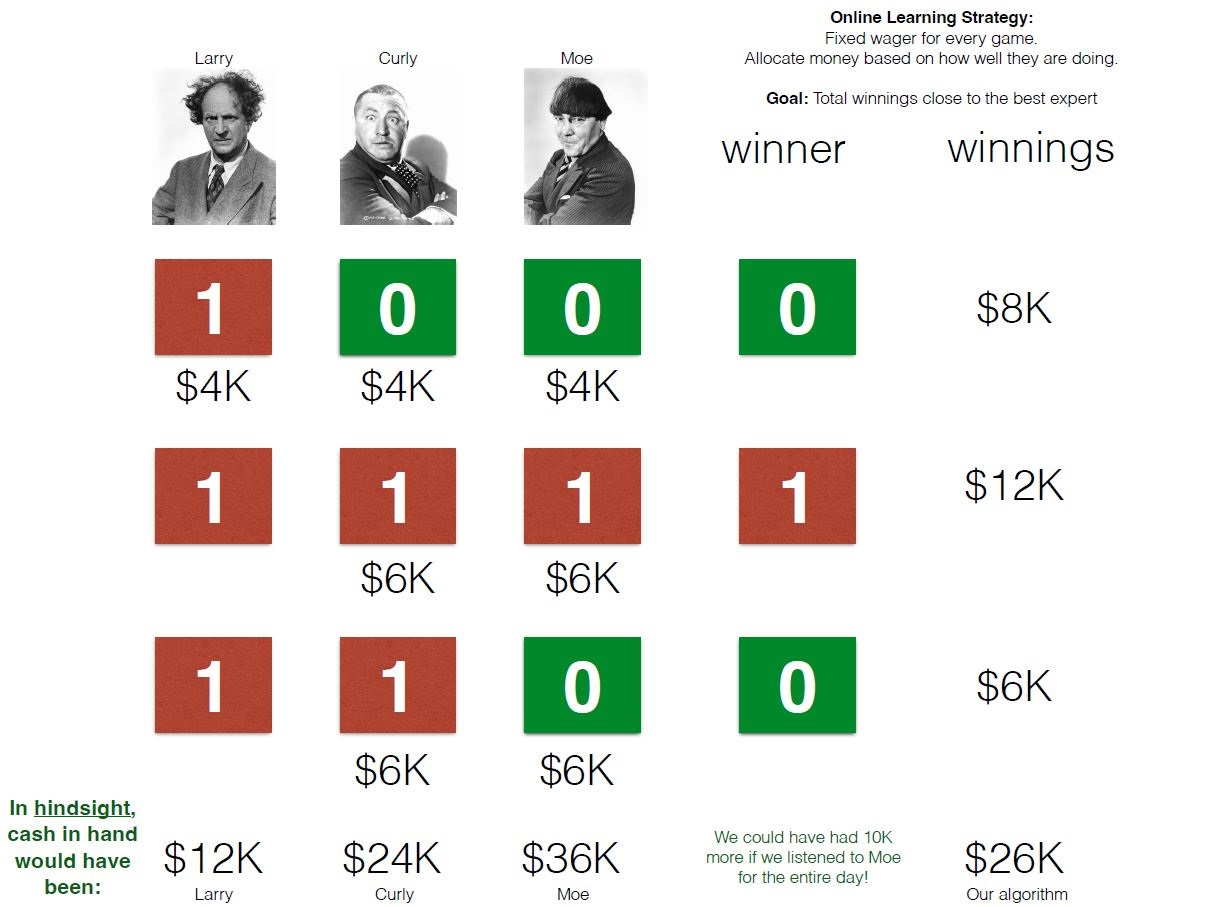
\includegraphics[width=4.5in]{pwea_gambling_example.JPG}
\caption{PWEA gambling experts example.}
\label{img:pwea-example}
\end{figure}

For a general PWEA method for this particular example, PWEA can be considered a one-shot, instructive, and exhaustive feedback method. Though the data samples are coming in as a stream, each round is not affected by the outcome of the previous race or the actions of the experts or learner, thus this is a one-shot feedback approach. The predictions of each expert are known and compared against, thus this is an instructive feedback approach. The action space is known to the learner, and one action can be analyzed against all possible actions the learner can take, thus this is an exhaustive feedback approach.


\subsection{Consistent (Greedy) Algorithm}

The greedy/consistent algorithm is a form of PWEA in which the algorithm determines the sole best expert by selecting the expert that has never been wrong. Essentially, the consistent (greedy) algorithm is a greedy method that finds the consistent, perfect expert. Thus, there is an underlying assumption that there exists a perfect expert somewhere in the set of experts, called the assumption of realizability which will be discussed later.

Figure \ref{img:consistent-greedy-example} shows the same scenario outlined in Section \ref{ssec:pwea-subsection} using the consistent (greedy) algorithm. Given no prior history of the experts, the learner randomly selects one expert and puts all the money onto that one expert's hypothesis. The end of the first rounds proves wrong for the selected expert, who has wrongly predicted the 1st horse to win. In the second round, the learner finds that the other two experts were right, and so the algorithm chooses the first available expert in the set of correct experts. The end of the second round shows that the 1st horse won again, so the learner continues choosing the first expert in the set because both continue to be consistent. In the third, the previously correct experts differ in their predictions, and the last expert comes out correct. So the learner finds that only the third expert has been the most consistent, and puts all money on the third expert's hypothesis for the next round. A similar comparison is performed at the end of the run, and the loss, or regret, is computed based on the winnings of the learner with the true answers to each of the rounds.

\begin{figure}[H]
\centering
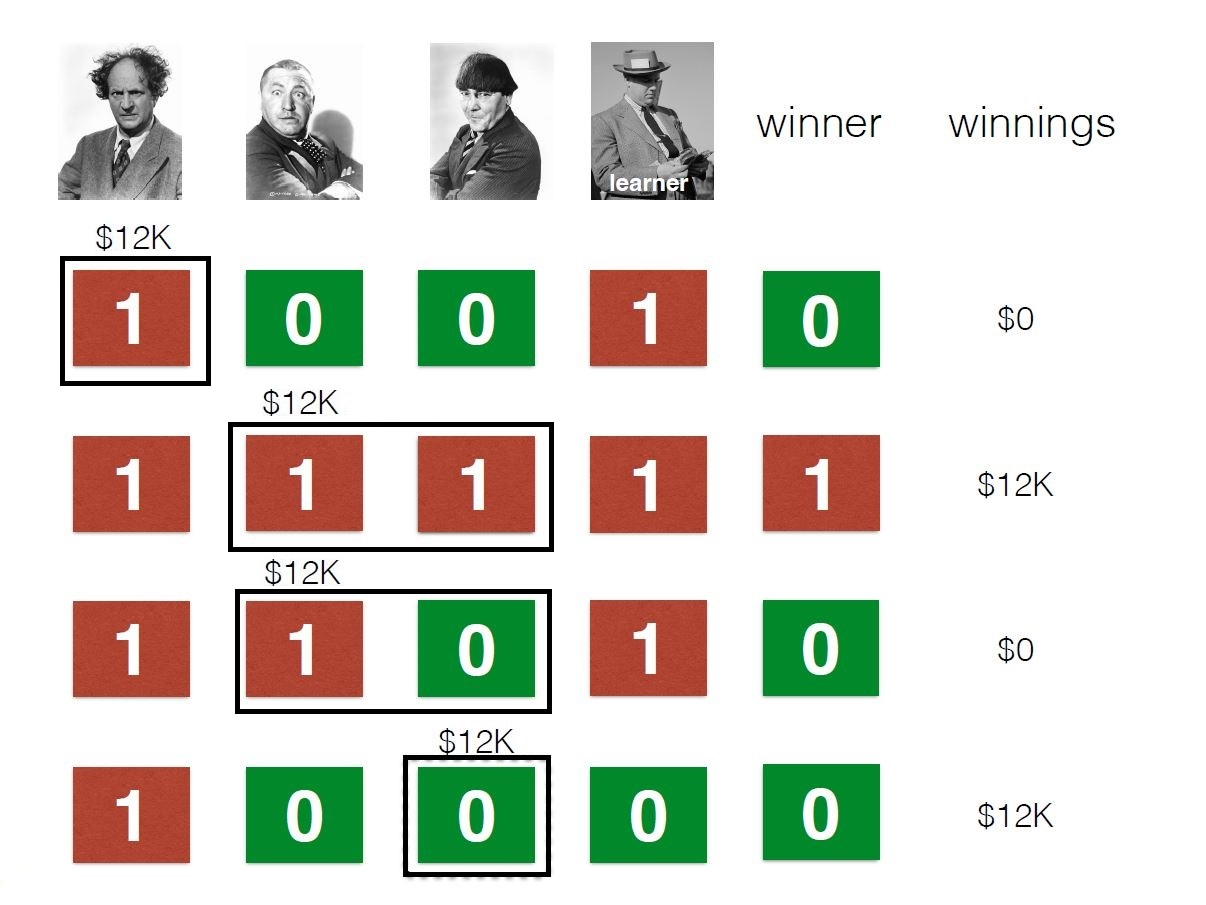
\includegraphics[width=4.5in]{greedy_gambling_example.JPG}
\caption{Consistent (Greedy) PWEA gambling example. }
\label{img:consistent-greedy-example}
\end{figure}

Given $X$ to be the set of possible observations (i.e. predictions from the experts), $Y$ to be the target domain set (i.e. true outcome from the horse race), and $H$ to be the hypothesis space mapping observations to the target domain (i.e. which experts will the learner choose to trust), the consistent (greedy) algorithm comes out as shown in Algorithm \ref{algo:consistent-greedy-algo}. Before the start of the algorithm's main learning loop, a hypothesis is extracted from the set of hypotheses, which in this case is the first hypothesis from the set. The last step of the algorithm's main learning loop is considered the update loop, which updates the hypothesis set to maintain only hypotheses that maintain the consistent experts so far in the learning loop. 

\begin{algorithm}[H]
\caption{Consistent (Greedy) Algorithm}
\label{algo:consistent-greedy-algo}
\begin{algorithmic}[1]
{\large
\STATE $\mathbf{V^{(1)}} = \mathcal{H}$  
\FOR{$t=1,\;\cdots,\;T$}
\STATE \textsc{Receive} ($\textbf{x}^{(t)}$)
\STATE $h =\textsc{FirstElem}(\textbf{V}^{(t)}) $
\STATE $\hat{y}^{(t)} = h(\mathbf{x}^{(t)})$ 
\STATE \textsc{Receive} ($y^{(t)}$) 
\STATE $\mathbf{V}^{(t+1)}\leftarrow \{ h \in \mathbf{V}^{(t)} : h(\textbf{x})^{(t)}=y^{(t)} \}$
\ENDFOR }
\end{algorithmic}
\end{algorithm}

Underlying the consistent (greedy) algorithm is the realizability assumption, which assumes there is a perfect, consistent expert within the set of experts. In other words, there exists a hypothesis $h^*$ in the hypothesis set $H$ such that $h^*:X->Y$. 

% \nocite{*}
\bibliography{refs} 
\bibliographystyle{abbrv}

%\section{Appendix}
%This section provides any relevant background material that was not covered in the lectures, but was found to be useful for understanding the material. 
%For example, derivations, theory underlying techniques employed, etc. 

%Additionally, this section can summarizes applications or extensions of these techniques found in the literature. 

\end{document} % Done!


